\chapter{El rostro contemporáneo del Estado moderno es el Imperio}
\label{cha:el-rostro}

Hemos señalado antes porqué el Estado opera también como maquina social. La máquina social codifica el deseo y el miedo de flujos descodificados. Quisiera recordar también que la latencia de los Imperios arcaicos da forma al Estado moderno. En ese sentido, el Imperio se caracteriza por la transformación de la publicidad al espectáculo y el advenimiento de las sociedades de masas, proceso relacionado con el auge de la radio y la televisión. En este capítulo me concentraré en explicar cómo se transforma el cinismo y la crítica del Imperio, fase contemporánea del Estado moderno. El Imperio es la máquina social orientada a la pacificación. Sigue con la misma estructura fundamental en su aparato de captura. A diferencia del Estado moderno, el Imperio no niega la existencia de la guerra civil, la gestiona. Se caracteriza por la informatización de la producción, donde la computadora es la herramienta \emph{universal} \autocite{hardtImperio2005} . En términos industriales, esta época se caracteriza por una transición del fordismo al toyotismo en la cadena de producción.

En quizá por la incorporación de las pantallas en la vida psíquica de los sujetos de Estado que las transformaciones del Estado son necesariamente transformaciones mediáticas. Si bien los medios no determinan, condicionan el desarrollo de la maquina social. Hardt y Negri también hacen hincapié en cómo la productividad, la riqueza y la creación de plusvalor toman la forma de una interactividad cooperativa a través de redes afectivas\rewrite{Me parece que esta mención es redundante, a menos que \enquote{comunicacionales y afectivas} sea una categoría diferente.}, lingüísticas, comunicacionales y afectivas \autocite[pp.~58,108]{hardtImperio2005}. A continuación presento la siguiente tabla para recapitular algunas cuestiones sobre lo interior y exterior del Estado como noología, como categoría del pensamiento \autocite{deleuzeMilMesetasCapitalismo2002}, que continuarán siendo de utilidad:

\begin{table}[htb]
  \caption{Leyenda} %Falta una leyenda en esta tabla así como un nombre que no sea tablename
  \label{tab:tablename}
  \centering
  \begin{tabular}{lcc}
    \toprule
    & \textbf{Interior} & \textbf{Exterior}\\
    \midrule
    \textbf{Modelo científico} & Compars & Dispars\\
    \textbf{Modelo jurídico} & Ley (logos) & Nomos\\
    \textbf{Forma ontológica} & Estado & Máquina de guerra\\
    \textbf{Modelo espacial} & Estriado & Liso\\
    \bottomrule
  \end{tabular}
\end{table}

En el capítulo anterior hemos desarrollado el argumento de que el Estado moderno es el fin de la guerra de religiones por la religión de Estado, además de explicar cómo la religión de Estado configura la subjetividad a través de la captura del deseo. Si bien el desarrollo del Estado obedece más a coyunturas sociohistóricas, la apropiación de toda técnica política y el hecho de que el desarrollo de las sociedades modernas esté condicionado a la economía de guerra, me obligaron a analizar desde un punto de vista de la estrategia cómo es que el Estado moderno logró llevar a cabo con relativa eficacia el proceso de pacificación histórica que dio forma al proyecto ilustrado del Estado universalista. Analizaré los mecanismos y las operaciones económicas sobre el deseo que permitieron al Estado moderno el gran avance que tuvo durante los siglos XIX y XX, que culminó con las dos guerras mundiales e implicó una transformación social a escala global a la que Tiqqun se refiere, en consonancia con los planteamientos de Hardt y Negri \autocite{hardtImperio2005} como \emph{Imperio}. Se trata, en principio, de un monopolio sobre lo político y sobre la crítica a través de la publicidad y la policía. Ahondaré en las tecnologías de captura que disponen a las formas de vida al arreglo mercantil de la sociedad y argumentaré cómo en el período de decadencia del Estado moderno, el capital produce nuevas formas de extracción que se asemejan al comportamiento de un virus informático, condición que permite que en el Imperio la soberanía se pulverice y las personas incorporen las normas sociales.

\section{Las formaciones sociales se configuran por procesos maquínicos y por ciertas capturas}
\label{sec:las-formaciones-sociales}

Según Deleuze y Guattari, la máquina social codifica el deseo. Esto quiere decir que las formaciones sociales se dan por procesos maquínicos y no tanto por los modos de producción. En el capítulo 3 de \emph{Salvajes, bárbaros y civilizados}, señalan que Estado viene de Marx ---modo de producción asiático---, Nietzsche ---origen y domesticación---, y Freud ---latencia---~\autocite{deleuzeAntiedipoCapitalismoEsquizofrenia2017}. El Estado despótico es \emph{Urstaat}. El Estado como máquina social consiste en una articulación doble. En lo social, un sistema institucional sociopolítico. En lo libidinal, un campo del deseo y de subjetivación. El capitalismo se sirve del \emph{Urstaat} como límite interior inhibido. El Estado capitalista conserva un vínculo con el despotismo, porque el capitalismo tiene potencias de muerte, derrama la antiproducción en la producción. Al final, la máquina social nunca funciona bien.

La formación asiática, la concepción de que el Estado surgió ya armado, está en la base, es el horizonte de toda la historia.

\begin{enumerate}[labelindent=\parindent, leftmargin=*, label=\roman*., widest=ii, align=left]
  \item El Estado despótico es el origen, es una latencia.
  \item El Estado es deseo de Estado.
\end{enumerate}

No hay más que el deseo y lo social, y el deseo forma parte de la infraestructura social. El deseo inviste el campo social, mediatizado por una instancia sociolibidinal de antiproducción: el \emph{socius}. \emph{Socius} está bajo las figuras de la tierra, el déspota y el capital. Ellas provienen de máquinas sociales diferentes.

Tanto la producción social como la deseante se articulan en distintos flujos de aparatos históricos de socialización del deseo. No son dispositivos lo que agencian y constituyen. Son los agenciamientos del deseo lo que expande las formaciones de poder. Los códigos sociales subordinan la producción deseante a las condiciones de reproducción de la estructura social. La producción deseante no solo es atravesada por códigos sociales, también por la emergencia de singularidades deseantes: figuras \hlfix{esquizias o n\'{o}mades.}{Tengo duda respecto al uso de la palabra \emph{esquizias}, parece m\'{a}s correcto usar \emph{esquicias}, pero no estoy seguro de lo que quieres decir con ella. Por otro lado, me parece que el plural de n\'{o}mada es n\'{o}madas.}

\begin{table}[htb]
  \caption{Leyenda} %Falta una leyenda en esta tabla así como un nombre que no sea tablename
  \label{tab:tablename}
  \centering
  \begin{tabular}{ccp{0.25\linewidth}}
    \toprule
    \textbf{Formaciones sociales} & \textbf{Máquinas sociales} & \textbf{Formas de Estado (motor inmóvil)}\\
    \midrule
    Salvajes & Territoriales/de linaje & La Tierra\\
    Bárbaros & Despóticas & Cuerpo del déspota\\
    Civilizados & Capitalistas & El capital\\
    \bottomrule
  \end{tabular}
\end{table}

Las formaciones no son progresivas, coexisten conformando una tipología social. El Estado despótico como \emph{Urstaat} es categoría y origen. La tarea principal de la máquina social es codificar el deseo y el miedo que generan los flujos descodificados. El Estado es una máquina en tanto que tiene un motor inmóvil y procede a diversas clases de cortes: extracción de flujo, separación de la cadena, repartición de parte. Las constantes de las máquinas sociales son represión general y registro de los flujos de deseo. Los géneros de registro-represión son:

\begin{table}[htb]
  \caption{Leyenda} %Falta una leyenda en esta tabla así como un nombre que no sea tablename
  \label{tab:tablename}
  \centering
  \begin{tabular}{ll}
    \toprule
    \textbf{Registro-represión} & \textbf{Sistemas}\\
    \midrule
    Codificación de flujos de deseo & Crueldad\\
    Sobrecodificación & Terror\\
    Axiomática de flujos descodificados & Cinismo\\
\bottomrule
  \end{tabular}
\end{table}

El capitalismo es la máquina social construida sobre flujos descodificados, sustituyendo códigos intrínsecos por una axiomática de las cantidades abstractas en forma de moneda. \emph{Urstaat} es el límite interior inhibido de la forma estatal capitalista: la máquina despótica, como origen reprimido, retorna en la máquina capitalista. Cada Estado histórico parece ser la reactualización de un Estado despótico, latente y supuesto en su carácter de originario o primordial. El Estado como categoría es un momento de abstracción, de idealidad y de trascendencia, es la dimensión objetiva de cada Estado histórico, incluido el capitalista. El Estado despótico (\emph{Urstaat}) es siempre origen y retorno. El primer movimiento de desterritorialización ocurre al \hlfix{otorgar a las comunidades territoriales}{¿Otorgar qué cosa?, parece que falta una palabra en esta oración.} como deuda infinita frente al déspota, padre o divinidad.

La máquina despótica es una megamáquina de Estado, pirámide funcional con el déspota en la cima como motor inmóvil. Los flujos codificados de este modo de producción asiático son sobrecodificados por la unidad trascendente que se apropia de la plusvalía. De esa forma, los imperios universales hacen camino al monoteísmo. Nietzsche señala: \enquote{en un mismo tiempo, la deuda infinita debe interiorizarse y espiritualizarse, la hora de la mala conciencia se acerca, será también la hora de mayor cinismo}. La latencia de Freud es un efecto demorado que explica cómo una tradición ignorada ejerce un afecto tan poderoso sobre la vida anímica de un pueblo. Los imperios arcaicos continúan estando presentes bajo las diferentes formas de Estados. La latencia se compone de \autocite{deleuzeAntiedipoCapitalismoEsquizofrenia2017}:

\begin{itemize}
  \item Fijaciones (existencia de una supervivencia de historias pasadas)
  \item Represiones/desalojamientos
  \item Retorno de lo olvidado (transformaciones, oscurecimientos, desfiguraciones)
\end{itemize}

Un ejemplo está en el lenguaje y el habla del Espectáculo sobre princesas, lo Real, las fantasías, etc. Los fundadores de un Estado operan la esencia interior, hacen una captura mágica. El Estado despótico es la formación de base, el horizonte de toda la historia. El carácter contingente y violento de su origen se recupera con la genealogía. El \emph{Urstaat} es una idea reguladora, principio de reflexión a partir del terror. No cesa de ser artificial pero se vuelve concreto mientras se subordina a las fuerzas dominantes. En su singularidad, el Estado despótico permite volver inteligible el mundo tal y como funciona el capitalismo y tiende a concretizarse en él.

Nietzsche señala que el Estado encierra al hombre-animal para domesticarlo. Opera una represión que lo vuelve hacia el interior de su vida, bajo las figuras de la culpa y de la mala conciencia. La voluntad del déspota (del padre) demanda la renuncia de lo \hlfix{pulsionar.}{¿pulsionar o pulsional?} La domesticación genera cierta satisfacción en el obedecer. La figura edípica se vincula con la deuda infinita, de modo que \hlfix{tanto m\'{a}s}{Si la frase \emph{tanto m\'{a}s} en esta oración puedes sustituirla por \emph{a lo sumo} sin cambiar el sentido entonces el uso es correcto, pero si lo que quieres decir es \emph{con mayor motivo}, entonces lo correcto es decir \emph{cuanto m\'{a}s}.} la reproducción social escapa a los miembros del grupo, más los vuelca en una reproducción familiar restringida y neurotizada de la cual Edipo es el agente. Se reprimen los flujos no codificados del deseo. Edipo codifica lo que escapa a los códigos, desplaza al deseo y a su objeto, sustituye la producción deseante por un sistema de creencias y de conciencia.

El déspota es un paranoico y sus burócratas unos perversos. (p.100)\addref{¿A qué referencia hace alusión esta página?} Él se retira de la vida de la tierra para jugar desde las alturas (principio de conocimiento paranoico). El déspota, el padre y la divinidad son la misma cosa, el ser objetivo y colectivo del deseo es el deseo \emph{del} déspota. El deseo del sujeto es \enquote{\emph{deseo del deseo del déspota}}. El cuerpo del déspota es la realidad libidinal del Estado, el representante del deseo inconsciente en esta formación social. Es el cuerpo pleno sin órganos. El Estado es también un agenciamiento.\footnote{Del Estado, sus burócratas y la agencia trataré en el Capítulo 4.} Es el acoplamiento variable de un conjunto de relaciones materiales y de un régimen de signos, la domesticación del deseo del animal-hombre y constitución de formas coloniales íntimas.

\subsection{El aparato de Estado cobra las rentas y reproduce la deuda}
\label{sub:el-aparato-de-estado}

En este apartado presento algunos esquemas sobre el aparato de captura del Estado. Recordemos que los dos mecanismos principales del Imperio son el Biopoder (mutación de la policía), que consiste en el traslado del orden de La Ley a la regulación a través de normas sin sujeto, interiorizadas. Mientras, el Espectáculo (mutación de la publicidad) consiste en la apropiación capitalista de la imagen para mercantilizar el deseo.\footnote{Más en el apartado sobre los monopolios y mecanismos del Estado moderno en este mismo capítulo.} Estos procesos maquínicos, que definen al Imperio como fase posterior al desarrollo e implosión de los Estados-nación, tiene distintos modos de regulación, que constituyen y dan forma a su aparato de captura \autocite{deleuzeMilMesetasCapitalismo2002}:

\begin{figure}[htb]
  \centering
  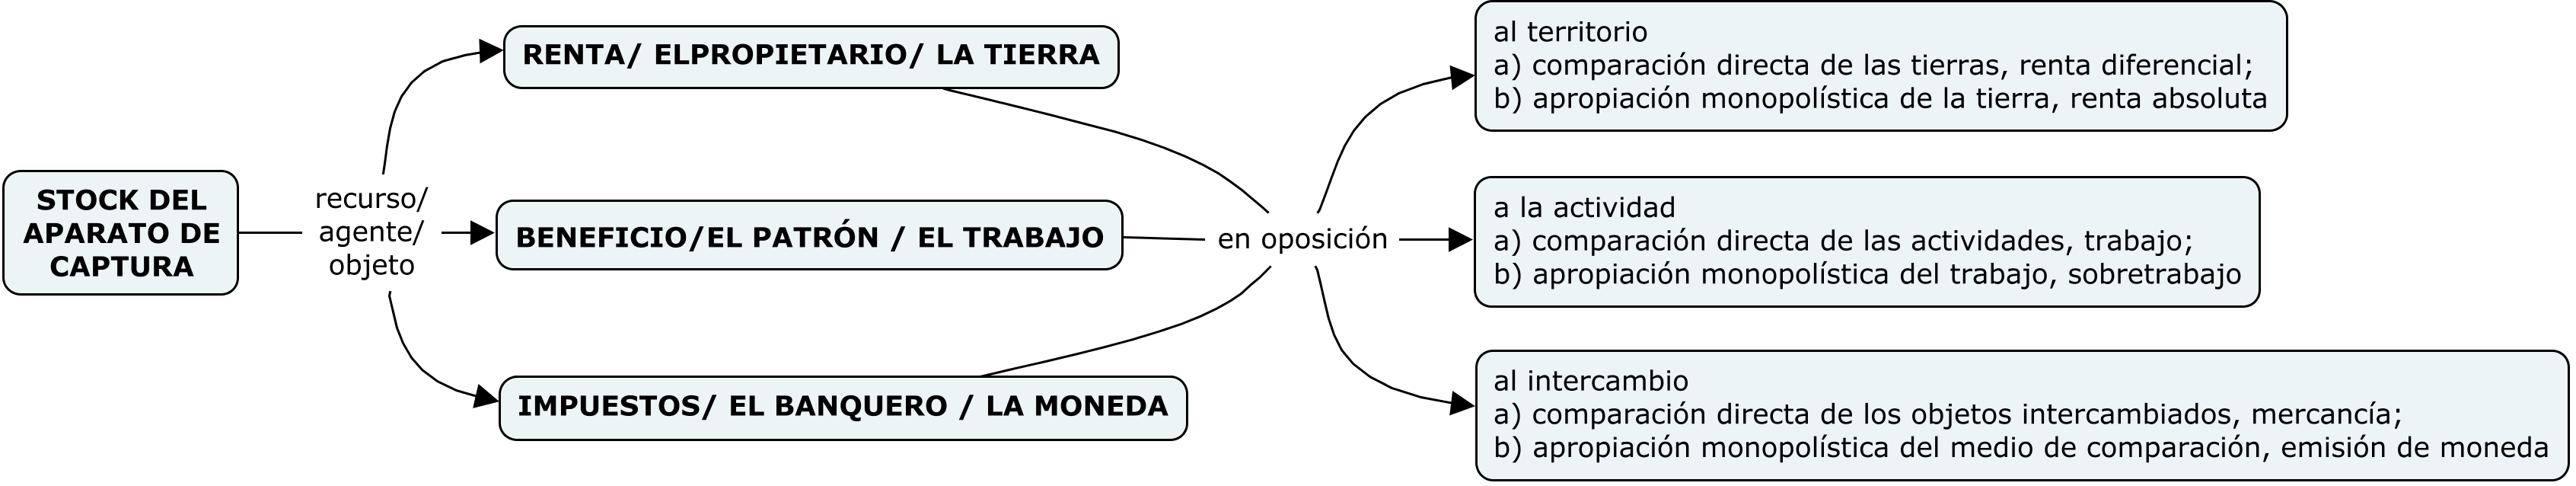
\includegraphics[width=0.7\linewidth]{images/deleuze-captura.png}
  \caption{Leyenda}
  \label{fig:deleuze}
\end{figure}

Por otro lado, la transformación del Estado moderno al Imperio se caracteriza por la sofisticación de los aparatos de captura en arquitecturas corporativas que bien podrían imaginarse como pirámides cristalizadas. Según el colectivo ANON, se trata de un arreglo piramidal donde la jerarquía y el conocimiento de formaciones sociales aumentan conforme se llega al tope de la jeraquía.

\begin{figure}[htb]
  \centering
  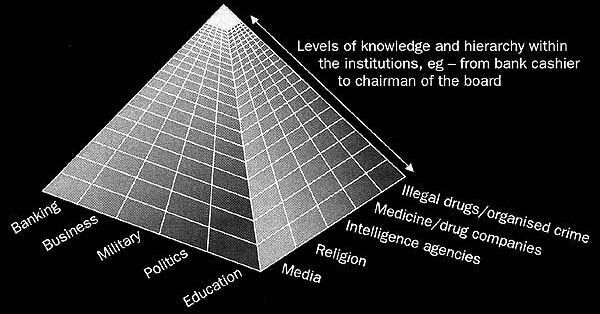
\includegraphics[width=0.7\linewidth]{images/knowledge-hierarchy-piramid.png}
  \caption{Leyenda}
  \label{fig:hierarchy}
\end{figure}

Al mismo tiempo, proponen una clasificación de los aparatos del Estado contemporáneo:

\begin{description}
  \item[Aparato socio-ideológico:] familia, tradición, religión, nacionalidad, etc. Codifica el deseo y la colonización psicológica del sujeto, establece hegemonía además de producir y mantener el estado actual de las cosas.
  \item[Aparato productivo-comercial:] finanzas, bancos, empresas corporativas, propietarios, etc. Comercialización de la producción, mercantilización del deseo para ligarlo al proceso de producción, monopolización del mercado, el valor de los desvíos que vuelve a los ricos a través de la parasitación de la mano de obra.
  \item[Aparato marcial-carcelario:] los militares, la policía, la inteligencia, el sistema de prisiones. Mantiene el estado actual de las cosas a la fuerza, la disciplina y el control de los sujetos, protege los intereses de los propietarios capitalistas y del Estado, sus fronteras, extrae recursos de otras regiones a través de la fuerza, redirige la riqueza para expandir el brazo militar del Estado e incentiva su investigación y desarrollo.
  \item[Aparato subversivo-periférico:] subjetividades colonizadas, grupos minoritarios, organizaciones criminales, la banda en sombra (\emph{shadow banking}), los mercados negros, etc. Muerte social y necropolítica. Establece la identidad de los ciudadanos mediante la otredad como diferenciación de subjetividades marginales, da un camino al lucro más allá del aparato comercial productivo.
  \item[Aparato legal de la soberanía:] el Estado, el sistema de justicia, los gobiernos, etc. Colonización el espacio geofísico, establecimiento del territorio y determinación de estratos y jerarquías sociales.
\end{description}

\subsection{Un dispositivo es la instancia molecular del aparato de captura}
\label{sub:un-dispositivo-es}

En la introducción planteamos que las resistencias no pueden encontrar soluciones a escalar molar, es decir global. Pese a lo aventurado de esa afirmación, lo cierto es que la vida interior de las resistencias está impregnada de deseo de Estado gracias a que el Estado como categoría del pensamiento ejerce su poder a escalar molar, y también molecular a través de la captura de la técnica política. En relación con el Espectáculo, el teatro de las operaciones del Estado moderno monta escenas, crea situaciones en las que existe una correspondencia entre objetos y su agenciamiento, es decir, aquello que se supone que se haga con el objeto. Un dispositivo es aquel objeto que cumple el fin para el que ha sido diseñado. Es más que una mercancía pues condiciona una respuesta más por una cuestión de diseño que de valor, como ocurre con las mercancías.

Antes de desarrollar los mecanismos del Imperio ---Biopoder y Espectáculo--- tenemos que precisar algunas cuestiones sobre los dispositivos. Dispositivo, según la definición de Foucault es un conjunto heterogéneo, que incluye virtualmente cualquier cosa, lo lingüístico y lo no lingüístico, al mismo título: discursos, instituciones, edificios, leyes, medidas de policía o proposiciones filosóficas. Es también una red de saber/poder, relación entre componentes institucionales. Tiene prácticas singulares cuya emergencia responde a un acontecimiento históricamente particular. Producen sujetos del saber-poder. Es un espacio de saber-poder donde se procesan prácticas discursivas y no discursivas. Producen los objetos de los que hablan (arqueología del saber) y sus regímenes de enunciación organizan las posibilidades de la experiencia (genealogía del poder), de acuerdo a condiciones de posibilidad dadas por la historicidad del acontecimiento. El dispositivo asigna al discurso a un sujeto para que garantice su implementación, en sí mismo es la red que se establece entre estos elementos, siempre tiene una función estratégica concreta y siempre se inscribe en una relación de poder. Es algo general, un \emph{reseau}, una \enquote{red}, porque incluye en sí la episteme, que es, para Foucault, aquello que en determinada sociedad permite distinguir lo que es aceptado como un enunciado científico de lo que no es científico. El dispositivo viene de la etimología \textsc{dis-positio}, \textsc{dis-ponere}. Los dispositivos están siempre en relación con una economía, un conjunto de técnicas para la conducción de instancias. El dispositivo se parece más a una configuración, a una instancia, a una implementación del pensamiento como construcción estriada del espacio. El dispositivo permite gozar de lo abierto como tal, del ente en cuanto ente más allá de la separación de los comportamientos animales de la vida del hombre. A la raíz está un deseo de felicidad. La captura y la subjetividad de este deseo en una esfera separada constituye la potencia específica del dispositivo. Según Deleuze, el dispositivo es una máquina para hacer ver y hacer hablar que se acopla a una historicidad de lo visible y lo enunciable, además de que el dispositivo produce subjetividad.

Para Agamben el dispositivo es positividad, un conjunto de significados impuestos al individuo desde el exterior. Un dispositivo es un ente con capacidad de normar a seres vivientes. Los objetos se vuelven dispositivos en cuanto forman parte de una red de saber-poder. Es un mecanismo que produce posiciones de sujetos por su disposición en red: el individuo es lugar de múltiples procesos de subjetivación. Lo paradójico es el cuerpo a cuerpo entre individuos y dispositivos, pues estos no solo subjetivan sino que producen procesos de desubjetivación, donde la creación de un sujeto implica la negación de un sujeto. Para el autor italiano, se trata de una teología económica y concibe a Cristo como el hombre de la economía (\emph{ho ánthropos tês oikonomías})\rewrite{Escribirlo en griego, ya que no se translitera.} de tal modo ser y acción, ontología y praxis están separadas por una esquizofrenia heredada a la cultura occidental. Bauman ha sugerido que la red que conforma a los dispositivos es un \enquote{sinóptico} que permite a muchos ver a pocos y es matriz donde se procesan a los sujetos consumidores de la sociedad del Espectáculo.

El dispositivo es un régimen social productor de subjetividad, de sujetos sujetados a un orden del discurso o cuya estructura sostiene un régimen de verdad. En la sociedad disciplinaria produce sujetos productores mientras que en la sociedad de control, sujetos consumidores. Todas estas subjetividades se integran según su capacidad de producir respuestas a sus interacciones o estímulos. Sin embargo, la subjetividad que está en disputa bajo el Estado moderno es el \emph{ciudadano-soldado-consumidor-espectador}, que es, en términos prácticos, el policía, el guardián de lo público. Es decir, es una unidad subjetiva modelada a partir del hombre blanco heterosexual con propiedades y en ese sentido construye un sujeto ideal estandarizado. Este sujeto es implementado como ideal a través de la industria farmacopornográfica. ANON propone una clasificación del dispositivo, que define como una disposición, como algo que hace hacer algo a alguna cosa. Sus prácticas son judiciales, tecnológicas y militares:

\begin{description}
  \item[Judiciales:] disponen determinadas \emph{decisiones}.
  \item[Tecnológicas:] los \emph{artefactos} están dispuestos de forma particular en sus piezas componentes o funciones de acuerdo a una disposición particular de estos mecanismos.
  \item[Militares:] ejércitos son dispuestos conforme a un programa estratégico para la \emph{batalla}.
\end{description}

Sin embargo, hay un afuera constituido por todas aquellas formas de vida que resisten a la lógica normalizante del Biopoder. En relación con el Estado, el afuera se encuentra en una reconfiguración del telos del Estado, de la necesidad a la crítica. En relación con las subjetividades, se trata de construir una subjetividad basada en el reconocimiento de la persona como forma de vida.

\subsection{El Estado moderno se vale de un doble monopolio sobre lo político y sobre la crítica, sus mecanismos son la publicidad y la policía}
\label{sub:el-estado-moderno-se-vale-de}

Los mecanismos de operación del Estado son la publicidad y la policía. La policía es la fuerza que interviene donde algo no marcha, donde un antagonismo entre \emph{formas de vida}, un salto de intensidad política ve la luz. La policía ha producido el espacio público como espacio cuadriculado, estriado, por ella. Así, el lenguaje del Estado se extiende a casi la totalidad de la actividad social y se transforma en el lenguaje social por excelencia. Si la política gira alrededor del interés, lo político lo hace sobre el deseo. Si la política es el libre juego del interés común, lo político es más bien el juego de significación de lo común en la vida. Para Rancière, la política va de la mano de la policía, de una forma de garantizar que existan agentes que desplieguen la fuerza física violentamente.\addref{Tal vez haga falta una referencia a Rancière en este punto.} Tradicionalmente este rol estuvo designado para la construcción del discurso público del urbanismo, práctica de gestión de las urbes. Recursos provenientes de estrategias militares de guerra fueron utilizados para el diseño de la segregación racial en ciudades como Chicago.\addref{Tal vez convenga añadir una referencia de este caso para ampliar la información acerca del caso de Chicago.}

La publicidad implica cinismo y la crítica es una forma de publicidad. Pensemos tan solo en el periódico, un medio desde el que podemos expresar diversas cuestiones sobre la crítica. Si el Estado se valió también del monopolio de la crítica es porque la crítica significó durante mucho tiempo lo que Tiqqun llama \enquote{el libre juego de las simulaciones}. La escritura pública, periódica, fue durante muchos años una cuestión propia de los ciudadanos. Es decir, de aquellos hombres que poseían los medios para \emph{hablar}. La publicidad consiste en la participación de los asuntos públicos, urbanos, y es la forma de agencia propia de la ciudadanía. La participación de lo público a través del periódico dió lugar a géneros literarios donde la burla del Yo y la total desconexión entre palabra y cuerpo es más palpable. De igual manera, con el desarrollo del periódico a la radio, a la televisión y algunos años después al internet, la forma que toma la publicidad se torna cada vez más espectáculo, representación convulsa de la imagen, disposición de la mirada al consumo del mundo, a su no participación de él. Así se configura una crítica espectacular, que construye elaborados discursos sobre el estatus quo que terminan formando parte de la industria cultural al no trascender la mera textualidad.

El monopolio de lo político exige también degradar la unidad diferenciada de un mundo en una nación, luego de esta nación en una población y un territorio, desintegrar toda la organicidad de la sociedad tradicional para someter los fragmentos restantes a un principio de organización, y finalmente, tras haber reducido la sociedad a una \enquote{pura masa indistinta, a una multitud descompuesta en sus átomos}, presentarse como el artista que va a dar forma a su materia bruta, y esto por el principio legible de la Ley. Queriendo concentrar el monopolio de lo político, ha politizado todo: todo aspecto de la vida se hizo político, no como contenidos singulares sino que, por la presencia misma del Estado, por su propia presencia, se constituyó a sí mismo en partido \autocite{tiqqunIntroduccionGuerraCivil2008}. En este contexto, la subjetividad que confronta Tiqqun con el Estado, los Bloom, ya no son sujetos, económicos, aún menos que de derecho. Se vuelven criaturas de la sociedad imperial, por lo que deben encargarse de ellos \hlfix{en cuanto que}{No es adecuado utilizar las expresiones \emph{en tanto} o \emph{en tanto que} con el significado de \enquote{en calidad de}, como usan muchos periodistas. Las formas \emph{en tanto} o \emph{en tanto que} equivalen en español a \enquote{mientras que}. Este error se debe al hecho de confundir \emph{en tanto} y \emph{en tanto que} con las expresiones \emph{en cuanto} o \emph{en cuanto que} que significan \enquote{en calidad de}.} seres vivientes para poder seguir existiendo \emph{ficticiamente} en cuanto que sujetos de derecho. Una contrahistoria desde el punto de vista de la guerra civil, permite verla como el progreso del monopolio estatal de lo político, victorias ganadas a un enemigo sin historia. La amenaza que representan estos enemigos es la de mundos autónomos, de colectividades no estatales.

El problema del agonismo de Mouffe tiene que ver con su legitimación del Estado y a que es hostil al control estatal, vuelve a plantear un espacio neutro que, sin embargo, siempre es una exterioridad en relación con el vínculo social. Los agentes de policía son aquellos a quienes se paga por consagrar todo su tiempo a cumplir los deberes propios de todos sus conciudadanos. Su misión está centrada en la resolución de los problemas (\emph{problem solving policing}) y preocupaciones de los ciudadanos. Ser policía es, según los grandes estadistas, un arte. De ahí la consagración casi espiritual de la sociedad y de las técnicas que perpetúan su existencia parasitaria. La salvación dejó de estar en el cielo para estar en la ciudadanía, en la entrega absoluta de todo vínculo al interés y a la necesidad. A un policía le encantaría ver cada rincón del universo como un espacio estriado, clasificado, cercado y con una base militar. Nada le causaría más placer que contemplar la metáfora schopenhaueriana de los puercoespines que se cubren del frío a la distancia porque si están demasiado cerca se insertan sus espinas. Y le gustaría verlo en todo el universo, o los multiversos. Es la manifestación de un espíritu totalitario, de una pretensión de reinar sobre todas las cosas, es la aspiración a la totalidad en un cuerpo que se halla alienado de la conciencia, que reconoce el concepto pero no es capaz de experimentar la unidad.

La construcción de la ciudad está relacionada con el desarrollo de la publicidad y la policía. Parece que el Estado, para hacerse más efectivo, se vale de una pragmática psicogeográfica. Es decir, una posición técnica orientada a la construcción de una percepción \emph{pública} del paisaje salvaguardada por un ejército de ingenieros, recaudadores de impuestos, vigilantes y personas dedicadas a la higiene de la ciudad. Pareciera que hay una suerte de similitud, al menos en lo que a públicos respecta, entre los manuales de la policía de Nueva York y los manuales de etiqueta de las cortes francesas en el siglo \textsc{xvi} \autocite{tiqqunIntroduccionGuerraCivil2008}. En relación con la ciudad, la dromología es el devenir arma de los medios de producción, el perfeccionamiento y la maximización de utilidades, la documentación de procesos y procesos de ingeniería iterativa para un balance entre plusvalor y utilidad. Es en este contexto cuando nace el Diseño como una heurística de la producción de mercancías.

\section{En el Imperio, la publicidad muta al Espectáculo y la policía al Biopoder}
\label{sec:en-el-imperio}

En este apartado abordaré algunas cuestiones básicas sobre la teoría crítica sobre el Imperio que desarrolla Tiqqun. Comienzo por la siguiente cita:

\begin{quote}
  Desde su nacimiento, la sociedad mercantil jamás ha renunciado a su odio absoluto de lo político, y es por mucho en esto que reside su mayor contrariedad: que el proyecto mismo de erradicarlo sea \emph{todavía} político. Desde luego quiere hablar de derecho, de economía, de cultura, de filosofía, de medio ambiente e incluso \emph{de} política, pero jamás de \emph{lo} político, dominio de la violencia y los antagonismos existenciales. A final de cuentas, la sociedad mercantil no es otra cosa que la organización \emph{política} de la negación desencadenada de lo político. [\ldots] La doctrina de la utilidad, el sistema de las necesidades, el mito de una autorregulación \enquote{natural} de los mercados, la ideología de los derechos del hombre y la democracia parlamentaria pueden ser incluidos entre los numerosos medios que fueron implementados en ese tiempo, para ese fin. Pero es indiscutiblemente en el período histórico que se abre en 1914 cuando la naturalización de la dominación mercantil reviste su forma más radical: el Biopoder. En el Biopoder, la totalidad social que se autonomiza poco a poco llega a hacerse cargo de la \emph{vida} misma. Por un lado, se asiste a una politización de lo biológico: la salud, la belleza, la sexualidad y la energía movilizable de cada individuo atañen cada año más claramente a la responsabilidad gestionaría de la sociedad. Por otro lado, es una biologización de lo político la que se opera: la ecología, la economía, la repartición general del \enquote{bienestar} y de los \enquote{cuidados}, el crecimiento, la longevidad y el envejecimiento de la población se imponen como los principales capítulos con los que se mide el ejercicio del poder. [\ldots] De lo que se trata en realidad, es de apoyar sobre la falsa evidencia del cuerpo y de la vida biológica el control total de los comportamientos, de las representaciones y de las relaciones entre los hombres, es decir, en el fondo, de forzar en cada uno el asentimiento al Espectáculo por medio de un supuesto instinto de conservación. [\ldots] el Biopoder es esa tiranía esencialmente asesina que se ejerce sobre cada uno en nombre de todos y de la \enquote{naturaleza}. [\ldots] No puede haber política \emph{en el seno} del Biopoder, sino sólo \emph{contra} el Biopoder. Considerando que el Biopoder es la negación consumada de lo político, la política verdadera tiene que comenzar por liberarse del Biopoder, es decir, revelarlo como tal~en~\autocite[Tesis V]{tiqqunTesisSobrePartido}.
\end{quote}

En el Imperio, la norma es el Estado de excepción. Es decir, el destino del Estado moderno no era otro que el de \enquote{nacer como el aparente vencedor de la guerra civil, para después ser vencido por ella. No haber sido más que un paréntesis y un partido en el curso paciente de la guerra civil} \autocite{tiqqunIntroduccionGuerraCivil2008}. La tensión propia del Estado moderno, es decir, su contradicción, yace en que el Estado se mantiene solo por la práctica de aquello que quiere conjurar, por la actualización de lo que supone ausente. Es evidente que la legitimidad del Estado radica de manera efectiva en sí mismo. El Estado en cuanto idea, como Dios, no requiere ningún tipo de justificación para existir. Su ideología es la que inventa las justificaciones como manera de posicionarse más allá de eso que ella misma ha construido. La modernidad creó al Estado y luego a la ciencia para inventar criterios que siempre se ejecutan por las instituciones. La ciencia y todo el discurso tecnocientífico capitalista crean límites, dicotomías, para asumirse como el eje sobre el que gira no solo su visión del mundo sino de lo real. En Tiqqun se plantea el despliegue del poder estatal como una pacificación. El Estado de excepción puede ser descrito como la paz en el Espectáculo, como la invisibilización de un montón de guerras que son libradas para mantener un orden, para contener toda potencia que puede desplegarse al caos, a lo múltiple, a lo íntimo \autocite[pp.~59-97]{tiqqunIntroduccionGuerraCivil2008}. El Biopoder es la sublimación del poder. El Imperio es inmanente a la sociedad, es la sociedad en tanto que esta es un poder. El Imperio tiene sentido solo a partir de la crisis, es decir, como negatividad. La respuesta del Imperio a la crisis es un estado de excepción. Las operaciones negativas, reactivas del Imperio a la crisis, son lo que evidencian su existencia. A diferencia del Estado moderno, El Imperio no niega la existencia de la guerra civil, la gestiona.

El Estado como estado de excepción tiene tanta necesidad de hacerse legítimo como \enquote{la Razón} en un mundo que no pide ser ordenado ni universalizado, que late en la inmensidad del infinito con tal facilidad que catalogarlo como caótico o armónico es una absoluta pérdida de tiempo. Sin embargo, el Imperio no rehúye de la Ley y La Institución. Las ve como armas, pero en realidad no conoce más que las normas y los dispositivos. El Derecho es un arma como cualquier otra en el despliegue universal de la hostilidad. Sin embargo, el Imperio siempre habla el único lenguaje que sabe hablar: el de la eficacia para reestablecer la situación normal, para producir el orden público, el buen funcionamiento general de la Máquina. Lo esencial no reside ya en una proclamación liminar de universalidad. La atención se apoya sobre las operaciones, sobre la \emph{pragmática}. Es una totalización que no nace ya de una voluntad de universalización: se hace por articulación misma de los dispositivos, por la continuidad de la circulación entre ellos. Es decir, del Estado moderno al Imperio, los fundamentos de Ley e Institución se transforman en normas y dispositivos, y la policía y la publicidad en Biopoder y Espectáculo.

En el Imperio, la publicidad se vuelve Espectáculo y la Ley se vuelve norma. La \hlfix{publicitaci\'{o}n}{¿qu\'{e} quieres decir con \emph{publicitaci\'{o}n}, ya que publicitar significa promover algo mediante publicidad y siento que quieres expresar que lo p\'{u}blico se vuelve privado.} es privatización, es un proceso de despojo donde se otorga a los negocios privados las redes de energía y comunicaciones que fueron construidas con \hlfix{gastos}{\emph{inversiones} sería un término más adecuado.} de dimensiones colosales con dinero público. Esa sutileza es lo que rompe el vínculo entre público y común para instaurar un régimen de lo público-privado, que será reforzado por la evolución de la publicidad en Espectáculo. Sin embargo, la propiedad privada también padece una crisis conceptual importante que, no obstante, no tiene implicaciones en la práctica (es decir, en los regímenes jurídicos y políticos). Se trata de un proceso de socialización que favorece al oligopolio de élite. En el Imperio ya no se trata de leyes sino de normas operando como agenciamientos. La norma ignora hasta la idea de una fundación. No tiene memoria, se mantiene en una relación muy estrecha con el presente, pretende desposarse con la inmanencia. En la norma reina una inaprensible instancia de totalización que disuelve, digiere, absorbe y desactiva \emph{a priori} toda alteridad. Bajo el régimen de la norma, nada es normal, todo está por normalizarse. Lo que funciona es un paradigma positivo del poder. La norma produce todo lo que es, en tanto que ella es \emph{ens realissimum}. La negatividad es tan solo un fallo respecto a la norma, un agujero en el tejido biopolítico mundial. Como respuesta, el Partido Imaginario es la sede de la potencia. La razón pública es, nuevamente, un momento, siempre ligado al trabajo, donde se le permite al ciudadano ser escuchado en lo público. Si el sentido común del ciudadano universal es la racionalidad, el mundo de las leyes y de imperativos morales que sirven únicamente como velos de cuanto dispositivo de control ha podido desplegar la sociedad. Esta supuesta racional estandariza todo anhelo y hace utilizable cualquier voluntad para alimentar la máquina de producción de deseo de la normalidad, del Estado para sí.

Habiendo señalado lo anterior, desarrollaremos el Espectáculo como despliegue de la publicidad. Para empezar, el Espectáculo introduce un problema: la dificultad para distinguir el deseo de la obligación. Se impone como obligatorio porque está en posición de ejercer el monopolio visual de la representación legítima. El novedoso principio de control convierte a cada cuerpo en un efecto de iluminación. La subjetividad en la época de la modernización capitalista está vinculada a aparatos modelizadores audiovisuales y estadísticos, propone una paradoja: no deja ver. Propone modos de ver dominantes y señala imágenes-tabú. La visión no es una mera actividad fisiológica social sino también un arte de ver para el cual es preciso educarse. El espectáculo inyecta dosis calibradas de goce y un atisbo del mundo redimido a través del consumo prometido. La esencia de las instancias del espectáculo no está en el análisis de su contenido sino en otras funcionalidades, como una red de relaciones en las que opera y su eficacia para organizar el campo de visión humano. Así, la cartografía territorial deviene atmósfera audiovisual. El espectáculo es una instancia del Estado y es un circuito de observación donde se observa y se es observado. Por ello, el Estado opera iluminando.

Después de las vanguardias, el espectáculo se obligó a renovarse a través de la mostración obscena de sus cimientos. Por ello, la parodia y el comentario infinito sobre sí mismo, además de la incorporación de nuevos productos paraculturales. En la ideología igualitaria del ciudadano se oculta el germen del despliegue masivo de la sociedad espectacular-democrática. La sociedad espectacular regula la circulación social del cuerpo y de las ideas. Nace con la modernidad para dar identidad y unidad a las masas con modelos culturales y funcionales a escala total. Espectáculo es la instauración de nuevas temporalidades y de inéditas topologías espaciales: ubicuidad espacial e intensidad y aceleración temporales, es una crisis de la flecha del tiempo. En todas partes, es diagramación de la mirada y transformación de la velocidad en tiempo inmóvil, el espectáculo es una fe perceptual. La cibernética crea tecnologías y burocracias especializadas en el arte de la vigilancia visual de los cuerpos. La misión de la sociedad tecno-espectacular no está en relación con el progreso sino en conducir a la humanidad a un estadio diferente de dominación, es una \enquote{imagen del mundo deseable}. Las metáforas de las patologías en el desarrollo tecnológico reproducen la lógica de sistemas corporales a las extensiones mediáticas (máquina infectada, contagio, virus). La reunificación de la comunidad es un movimiento inventivo de sí mismo. Y la sociedad comunicacional su negación. Lo que es \enquote{real y experimentable} no puede ser \enquote{representado ni interpretado}.

La cultura espectacular desorganizó la antigua unidad de la clase trabajadora basada en una cultura festiva común. La administración del territorio siempre ha necesitado del arte político, de la desorganización de la comunidad con escribas, burócratas, legitimadores, asesores, parlamentarios). Esto se combate con amistad política. En otras imágenes de sociabilidad nos encontramos con la vindicación de la fiesta y el banquete, y el rechazo a la \hlfix{cotidianidad}{Aunque tanto \emph{cotidianidad} como \emph{cotidianeidad} son términos válidos para referirse a la cualidad de cotidiano, se prefiere la primera por ser la formación regular a partir de \emph{cotidiano} no cotidianeo.} alienada y al trabajo. El espectador se licúa en una pasividad, crueldad morbosa activa ante la contemplación en diferido de la persecución de sufrientes y perseguidos. Hombres libres son aquellos curiosos que lanzan sondas hacia lo todavía invisible o inaudible.

Lo espectacular integrado es la superación del poder espectacular concentrado (que prioriza la ideología del Estado totalitario como verdad) y el difuso (prescribe la elección deliberada de una variedad de mercancías). Se combinan a través de la renovación tecnológica, fusión económica entre lo público y lo privado, imposición de un verosímil que no admite réplica y la abolición de la memoria histórica, además del exilio de toda forma no espectacular. A estos enemigos se les combate haciendo silencio a su alrededor.

\subsection{El posfordismo es la informatización global del trabajo}
\label{sub:el-posfordismo-es-la-informatización-global-del-trabajo}

\epigraph{\enquote{La tecnología es un discurso sobre las técnicas que no cesa de realizarse. Así como la ideología de la fiesta es la muerte de la fiesta real y la ideología del encuentro es la imposibilidad misma del encuentro, así la tecnología es la neutralización de todas las técnicas particulares. El capitalismo es en este sentido esencialmente tecnológico; es la organización rentable, en un sistema, de las técnicas más productivas. Su figura cardinal no es el economista, sino el ingeniero.}}{\emph{El Comité Invisible} en~\autocite[p.~131]{comiteinvisibleNuestrosAmigos2015}.}

Dicen Hardt y Negri que el declive de la legitimidad de los Estados nación no significa necesariamente un declive en la soberanía. Habría entonces que comprender la evolución de nuestro concepto considerando la nueva dinámica de producción de poder en la sociedad contemporánea. \emph{La libertad se antepone al orden en las sociedades disciplinarias y a la gestión en las sociedades de control.} Esta idea de control reproduce la cuestión de un capitalismo de medidas, de una fase del capitalismo cuyo hito se encuentra en la cibernética como ciencia y arte del control. El Imperio despliega dispositivos de regulación normativa y biopolítica que se extienden hacia muchas partes pero tienen veracidad en cuanto a que producen ciertos flujos de información. Sus aportes permiten entender la cuestión desde una lógica económica. Para ellos, el Imperio es una nueva forma global de soberanía, un aparato de regulación descentralizado y desterritorializante. Cada Estado nación es un Leviatán. La posmodernización de la economía global tiende a la producción biopolítica. Ni Estados Unidos ni otro país están en el centro del proyecto imperialista. El Imperialismo ha terminado. Sin embargo, Estados Unidos tiene fundamentos imperiales, al contar con una constitución formal, compuesta por la Constitución política y otros aparatos legales, y una constitución material, que no es otra cosa sino la formación y reformación de la composición de las fuerzas sociales. Estados Unidos sienta las bases de un arreglo estatal distinto al de los anteriores, donde las contradicciones entre Imperio y República en \autocite[Tratado de Nomadología]{deleuzeMilMesetasCapitalismo2002} fungen más bien como una tensión vital, a diferencia de los arreglos de Europa y su interminable guerra de religiones. \emph{The Federalist}, escrito por Thomas Jefferson, propone abiertamente un concepto, aunque las más despistadas lo miren como una metáfora.\addref{Jefferson, si es que no está mencionado en la siguiente referencia de Hardt y Negri.} Se refiere a un agenciamiento que suspende la historia. Regula no solo las interacciones humanas sino también la naturaleza humana, es la forma paradigmática del biopoder, su fin es la paz perpetua en la historia~\autocite{hardtImperio2005}.

La informatización de la producción está relacionada con el desmantelamiento de la fábrica. Desde su ámbito más productivo, el Imperio puede comprenderse como parte de un proceso económico de informatización de la producción. Hardt y Negri hacen uso de una metáfora sobre la fábrica para explicar las asimetrías históricas entre los países frente a la idea de desarrollo económico. Parten de la premisa de que la producción de un Estado pasa por una fase de agricultura, industrialización y, en estos tiempos, de informatización. A diferencia de lo que predican los \hlfix{ap\'{o}stoles}{La acepci\'{o}n de sacerdote en español no parece admitir este uso, que sin embargo s\'{\i} recoge el vocablo ap\'{o}stol para referirse al \emph{propagador de cualquier ideolog\'{\i}a o doctrina}.} de la Economía, estos procesos no son escalonados y su anacronismo ignora que hay ventajas permanentes que prevalecen, como el uso político de la palabra, que bien puede traducirse en las capacidades de otros cuerpos políticos para el libre juego de las formas de vida. La cuestión más concreta, en el caso del Derecho internacional tiene que ver con el derecho a explotar la propiedad, extendiéndose ésta hasta el ámbito de los saberes y de las técnicas de exterioridades, que permitan dar más vida, aunque sea artificiosa, al soplo del Leviatán. La falacia ignora que no en todos los países se completa un estadio de modernización (en términos de producción) antes de pasar al siguiente y ofrecen el caso de Italia como ejemplo, que es poderosa en productividad, pero solo en la medida en que conviene a la inversión extranjera. En lo que respecta a las fronteras territoriales, el Imperio las convierte en aduanas-volantes. Un ejemplo claro es el espacio Schengen, que designa el territorio de libre circulación al interior de la Unión Europea. Las aduanas se extienden, en potencia, a todos los lugares y a todos los instantes. A diferencia del Estado moderno, que opera apelando a la Ley y la Institución, el Imperio es el garante de la proliferación reticular de normas y dispositivos. El Imperio calcula, pesa, evalúa y luego decide estar presente en un lugar o en otro. Manifestarse o retirarse en función de consideraciones tácticas. De modo que está en donde podría estar. Se mantiene en cada punto del territorio, en el espacio que hay entre la situación normal y la situación excepcional, puede su propia impotencia.

El Imperio se caracteriza porque su modo de producción da forma a una inteligencia cibernética de las tecnologías de la información y de la comunicación. La consecuencia más importante de esto tiene que ver con una transformación en la concepción del trabajo, que a su vez afecta el modo como se comprenden la tierra y el capital como factores restantes de la producción. Este cambio paradigmático consiste en la transición del fordismo al toyotismo. Por la abstracción del trabajo, fragmentado a través de diferentes actividades, la computadora se propone a sí misma no solo como central sino como \emph{herramienta universal}, a través de la cual pasaría toda actividad. Significa también un trabajo afectivo e inmaterial, que produce redes sociales, comunidad y Biopoder. El trabajo inmaterial del sector de servicios tiene que ver con la manufactura, con tareas analíticas y simbólicas, y la producción y manipulación del afecto a través del contacto humano.

En términos históricos, el futuro del trabajo empieza en Japón. A fines de los años setenta y a lo largo de los ochenta, con el declive del fordismo-taylorismo, experimentamos un auge del toyotismo. Este viraje coincide con el auge de la literatura gerencial y su gran auge como \emph{best-sellers}. Esta forma de literatura narra la evolución y configuración del futuro del trabajo. El sistema de información de las nuevas líneas de ensamblaje, desarrolladas en Toyota por Taiichi \={O}no, plantea una producción en serie distinta al modelo fordista tradicional. La distinción está en el \emph{push-pull}. En la cadena de suministro \emph{push}, o de empuje, la producción se determina por la planeación, mientras que en \emph{pull}, por \hlfix{jaloneo}{Esta traducci\'{o}n me parece desafortunad y poco clara, porque el sistema Toyota plantea un \emph{pull system} que ser\'{\i}a m\'{a}s bien un sistema de control dentro del proceso de producci\'{o}n que significa solicitar las piezas que se necesitan, cuando se necesitan y en la cantidad exacta necesaria, para evitar mermas.}, está determinada prácticamente por la relación entre oferta y demanda. Esto favorece el proceso de pulverización del ensamblaje de mercancías, simplificando y exacerbando al mismo tiempo la enajenación del trabajador. Este modelo ha mutado para adaptarse a las dinámicas tecnocapitalistas que predominan en el cínico ambiente de la innovación tecnológica, donde abundan las formas cibernéticas de producción y de control colaborativo. El desencanto de la élite neorreaccionaria de Sillicon Valley se exacerba, como hemos visto anteriormente, \hlfix{cuanto m\'{a}s}{Este es un uso leg\'{\i}timo en el habla de M\'{e}xico y parte de Centroam\'{e}rica, pero es en un registro coloquial, por lo que es preferible emplear \emph{cuanto m\'{a}s} que es la forma escrita más extendida en la hispanidad.} aguda es la alienación, cuanto más\revstyle{Ibid.} potente es la tecnología para automatizar tareas.

La fuerza de trabajo es capital variable, una fuerza activada y configurada solo por el capital, porque los valores cooperativos de la fuerza de trabajo, particularmente el trabajo inmaterial, le permite al trabajo valorarse a sí mismo. De modo que hoy, la productividad, la riqueza y la creación de plusvalor toman la forma de una interactividad cooperativa a través de redes afectivas, lingüísticas, comunicacionales y afectivas. Lo anterior muestra de qué modo la dualidad conceptual que existe entre el trabajo y el ocio son síntomas del Biopoder. Los avances de la cibernética desterritorializan la producción dispersando las fábricas masivas, evacuando las ciudades-fábrica, pues para el patrón comienza a resultar innecesario tener una fábrica cuando el \emph{coworking} y las oficinas-café pueden cumplir esa función. La cadena de ensamblaje es reemplazada por redes, sin centro físico o territorial. Dejando atrás los modelos verticales, industriales y corporativos, la producción está organizada en redes de empresas horizontales. La informatización de la producción y la importancia de la producción inmaterial permiten liberar el capital de los límites tradicionales de territorio o de negociación. En clara afinidad con los planteamientos de Paul Virilo, Hardt y Negri apuntan hacia las carreteras como caminos romanos, donde la paradoja reside en que la red en sí misma es al mismo tiempo el sitio de producción y de circulación \autocite{hardtImperio2005}. Así, el Estado moderno logra consolidar la tensión entre Imperio y República a través de un mecanismo democrático, el internet como rizoma, y uno oligopólico, una red de transmisiones y difusión de la industria de la cultura, algo que ellos llaman una nueva estructura híbrida de información-red.

En el posfordismo, la gestión de la vida y la muerte es cibernética, pues nuestro mundo es de redes, navegable a través de teorías de la complejidad y del caos. Muchos procesos automáticos alimentan diariamente el flujo de operaciones de las infraestructuras (redes de abasto de combustibles, electricidad para servidores, satélites, líneas de internet) sin que haya realmente un responsable. Las funciones están programadas y los destinos predeterminados. Miles de variables interactuando entre ellas a partir de distintos nodos que envían información diversa y que demandan u ofertan certificados, \hlfix{\emph{requests}}{¿qu\'{e} quieres decir con esta palabra en este punto?}. El propósito de la cibernética es dispersar para crear un caos gestionable, incluso automatizable. Ella condiciona una nueva relación ontológica, un \emph{gestell}, entre las formas de vida y las cosas a través de la imagen, con el auge de la sociedad red y gracias al desarrollo acelerado del internet. Si el Estado moderno reina sobre la república fenoménica de los intereses, el Imperio reina sobre la república fenoménica de las diferencias, es en realidad el libre juego de los simulacros. La idea democrática de la equivalencia entre todas las formas de vida no es distinta de la idea imperial. De modo que la democracia es imperial al establecer la equivalencia negativamente, por el hecho de impedir por todos los medios que las diferencias éticas alcancen en su juego el punto de intensidad en que devienen políticas. La república política es la democracia en el interior de la forma abstracta del Estado. Es por eso que la forma abstracta de Estado de la democracia es la República. En la verdadera democracia, el Estado político (en la medida en que apunta a la ficción de lo Uno real y toma partido por ello, neutralizando su uso metafísico de las técnicas) desaparecería. El capitalismo es el arma técnica-productiva del Estado y el patriarcado el referente simbólico, mientras que el Estado se refiere solo al proceso, es noología ante todo. La cibernética se entrecruza con la inteligencia y la farmacopornografía a través de técnicas masturbatorias, donde toda producción cultural es entretenimiento. Parece que hay una forclusión de la potencia gaudendi (véase~\ref{wrd:potentia}) por la creación de ciertos soberanos legítimos con el monopolio de la excitación.

El arma más letal y compleja del Imperio es la cibernética. Si aceptamos la metáfora ciborg de Haraway y asumimos que somos, al mismo tiempo, organismo y máquina, nuestro cuerpo es complejo entramado de canales y circuitos susceptibles de ser penetrados. Podemos definir a la cibernética como ciencia y arte del control.

La teoría de la información es uno de los elementos centrales de la cibernética. El dominio tecnológico de esta para el mundo yace en la capacidad de instrumentalizar cualquier relación. Entender los circuitos de información se hace clave para ir más allá de la visión tecnologizante de la realidad, para encontrar mecanismos que rompan la lógica de control que se hace cada vez más difusa y permanente dentro de la vida. La \emph{forma de vida} que por su comprensión tecnocrítica del mundo es capaz de desdoblar y visibilizar los elementos que dan poder al Imperio en su despliegue cibernético, es una que deviene hacker. La constitución de una multitud de hackers constituye un cuerpo político pirata. Es necesario que mencionemos que este espíritu es también el más proclive a entregarse al Imperio si este logra sembrar la necesidad en el espíritu. De suerte que el hacker se encuentra siempre en un dilema de acción, pues en cualquier momento puede volverse un policía. Y no solo eso. Es tan fino el saber del hacker que su traición podría significar aumentar su potencia al grado de volverlo un robocop: policía de lo real en el deseo.

La descentralización ha sido una de las herramientas más poderosas e invisibles del Imperio para la difusión de su poder. Hardt y Negri explican cómo la desterritorialización permite que el dominio biopolítico de este Leviatán sea cada vez más sutil. Frente a ello, el paradigma de redes distribuidas se asemeja más a la posibilidad de crear un mundo de autonomía, con saberes relativamente accesibles, donde no hay centros de poder porque todo está, literalmente, en todas partes.

La cibernética nos ha convencido cada vez con menos argumentos y dificultades, de la importancia de vivir siempre a expensas de una moneda con la intención de reproducir el dominio de la Publicidad en toda relación, de tal suerte que el Espectáculo pueda mantenerse como el dominio pleno de lo real. Queda así como un tema de suma importancia la distinción entre lo real, lo virtual y lo digital.

En lo que respecta al deseo, consideremos en principio lo siguiente: el Imperio no solo genera un despliegue biopolítico de poder, sino que también desarrolla, cada vez con más eficacia, una cibernética del deseo. Una de las formas más simples para entender la naturaleza de esta cibernética del deseo la plantea \autocite{preciadoTestoYonqui2008} con el concepto de \setconcept{\emph{potentia gaudendi}}{wrd:potentia}. Esta potencia es una que atañe a la libido y que evidencia de manera concreta la tesis de Deleuze sobre la producción-deseo. Entre otros problemas, uno de los principales desafíos es cómo crear una relación dialéctica entre lo común y lo íntimo que rompa con la lógica de lo público-privado.

Los desarrollos de las nuevas ciencias, en particular en teoría de redes y cibernética nos permiten entender los sistemas de maneras muy distintas y con problemáticas que también difieren. Por un lado, pese al miedo que la izquierda más dogmática y que una misma rama de sombra ludita dentro del anarquismo radical tienen frente a la tecnología y al control, no reparan en que el problema es la tecnología como concepto. En el Espectáculo, en lo que en Tiqqun denominan como época de la indeterminación, del \emph{se}. En el siguiente apartado desarrollaré la cuestión de las tecnologías cibernéticas y su relación con la producción cultural.

\subsection{La industria farmacopornográfica es el paradigma de toda industria cultural}
\label{sub:la-industria-farmacopornográfica}

\epigraph{\enquote{Todas las razones para hacer una revolución están ahí. No falta ninguna. El naufragio de la política, la arrogancia de los poderosos, el reinado de lo falso, la vulgaridad de los ricos, los cataclismos de la industria, la miseria galopante, la explotación desnuda, el apocalipsis ecológico\ldots{} no se nos priva de nada, ni siquiera de estar informados de ello. [\ldots] Todas las razones están reunidas, pero no son las razones las que hacen las revoluciones; son los cuerpos. Y los cuerpos están delante de las pantallas.}}{\emph{El Comité Invisible} en~\autocite[p.~7]{comiteinvisibleAhora2017}.}

La forma despótica del Imperio se caracteriza por una pulverización del poder y un cambio en los modos de producción, donde se privilegian los procesos industriales pulverizados, sin fábricas ni obreros reunidos en un mismo espacio, también por el auge de entidades más allá de los Estados nación, como las empresas trasnacionales, que compran representantes políticos en Cámaras legislativas y parlamentos para legislar en favor de sus intereses. Detrás de cada uno de los aparatos de Estado existen entidades económicas con transacciones y reglas del juego que regulan la vida en diferentes esferas pero a dos escalas, una micro (corporal, que corresponde al Biopoder y el Espectáculo) y macro (burocrática, de legislación e infraestructura tecnológica). En principio, podríamos hablar de las cinco grandes empresas que condicionan el desarrollo de las telecomunicaciones: Google, Apple, Facebook, Amazon y Microsoft (\textsc{gafam}). Estas son la base material por donde fluyen información y códigos sociales, representaciones del mundo, que son reproducidas en los dispositivos personales para provocar una reacción, un deseo. Esta nueva forma del capital explota reacciones, capitaliza el placer que puede cuantificar en \emph{clics} y \emph{shares}.

Este ciclo se basa en un delicado circuito de excitación, frustración y excitación que regula los hábitos de consumo. Se trata del modelo ideal de empresa neoliberal, un paradigma del negocio posindustrial. La pornografía es un régimen estético que produce significados y un modo de presentación de las cosas que resulta adictivo, que permite obtener satisfacción del placer masturbatorio sobre la representación de cualquier fantasía posible materializada en videos.\footnote{De cierto modo, que el capitalismo se presente actualmente en su mayor apogeo a través de la industria farmacopornográfica (régimen toxicológico y semiótico-técnico), reproduce una concepción de la subjetividad como no castrable, cuyo horizonte parece ser el de autómatas dependientes del \emph{soma} de Huxley, personas discapacitadas, incapaces de habitar, de subsistir autónomamente. Cfr. \autocite{preciadoTestoYonqui2008}.} En los foros de internet para varones adictos a la pornografía existe un nombre para el circuito pornográfico que tiene atados a tantos hombres a una forma particular de desear. Se conoce como: \emph{Porn, Masturbation, Orgasm (PMO)} \autocite{NoFapDonLie}. El malestar de estos hombres cada vez más incapaces de vivir y en simbiosis con las comodidades del capitalismo que extienden el poder de sus formas tristes de vivir a otras esferas sociales, son el síntoma de este nuevo rostro de la economía. La excitación, la erección, la eyaculación, el placer y el sentimiento de autocomplacencia y control omnipotente se vuelven materias primas del proceso productivo.

Por esta razón, Paul Preciado señala que la pornografía es el rostro desenmascarado de la industria de la cultura y propone el concepto de \emph{farmacopornografía} para referirse al gobierno biomolecular y semiótico-técnico de la subjetividad sexual. Hay, de hecho, empresas que se encargan de regular la producción de contenidos excitantes que funcionan como mercancías con estudios explotadores y personas trabajadoras sexuales explotadas. La explotación mercantil del sexo es paradigmática porque un solo video puede producir millones de orgasmos \autocite{StatsArchivesPornhub}, lo que contrasta con la industria farmacéutica, donde el desarrollo de un medicamento cuesta muchísimo pero es fácilmente reproducible una vez que se obtiene y patenta una fórmula \autocite{preciadoTestoYonqui2008}. Así, las grandes entidades económicas capitalizan problemas clásicos de la economía como las asimetrías de información, el problema de agencia o los dilemas de acción colectiva. Además, condicionan nuestros deseos imprimiendo en nuestras psiques imágenes de lo deseable, además de crear una erística que nos enseña que esos estímulos que aprendemos a desear los podemos obtener a través de la moneda, de intercambios mercantiles. Estas empresas aprenden a través de costosas investigaciones sobre el comportamiento humano, para reproducir la servidumbre en los contenidos a través de segmentos de mercado donde se puede insertar el discurso del parásito capitalista bajo distintas situaciones y formas sexuales. PornHub es el paradigma de la industria cultural por su capacidad para producir orgasmos, para \emph{gestionar el género, la excitación, la frustración y el placer}. De este modelo de empresa se pueden extender otras versiones blandas (\emph{soft}) que operan en otros aparatos sociales. Por ejemplo, Disney funciona como el dispositivo que reproduce el imaginario de la jerarquía social a través de sus mitos de princesas, reyes y la construcción del otro como monstruosidad. Algo parecido hacen McDonald's y Coca Cola para reproducir la chatarrofagia.\footnote{Es decir, la enfermedad de la impotencia, del cuerpo enfermo, pauperizado, envenenado por las bombas mediáticas que producen la comida rápida o chatarra como lo deseable, como el lugar donde gastar el \emph{salario}. Se trata de un régimen alimenticio de productos vacíos, compuestos de harinas, grasas, sodio, azúcares y otras sustancias que funcionan bajo el mismo principio de estimulación-malestar y que producen serios daños al cuerpo a largo plazo. El paradigma mercantil de la comida en tiempos del Imperio.}

En el Imperio, que es la crisis del Estado moderno, es decir, la crisis de la religión de Estado, el capitalismo se comporta como un virus. El cambio de paradigma de modelos de gobernanza en masa a modelos en red obedece al desarrollo cibernético del algoritmo\revstyle{¿cuál de todos los algoritmos?}. Las sociedades disciplinarias y de control son demasiado complejas para gestionar, por lo que es más fácil fijar protocolos para gestionar redes de manera más eficiente. El espacio masivo está condicionado al número de participantes en un espacio y un momento particulares mientras que el espacio de redes se extiende y contrae en el espacio-tiempo de acuerdo a las órdenes y necesidades de la red. Es decir, su uso del capital es más eficiente porque se ajusta a las necesidades de cada momento. La economía posfordista computacional se basa en circuitos de producción de excitación-frustración y el porno es el paradigma de la industria cultural porque permite transformar cualquier pulsión en mercancía capitalizable a través del \emph{tracking} (seguimiento) del tráfico de sus efectos frente a los espectadores. La excitación, la erección, la eyaculación, el placer y el sentimiento de autocomplacencia y control omnipotente se vuelven materias primas del proceso productivo. Los reaccionarios son peligrosos porque son los consumidores y espectadores de la farmacopornografía. NRx\todo{Tal vez sea necesario añadir una nota que explique qué o quienes son NRx.} transforman concienzudamente todas las transacciones en utilidad.

Parece que en tiempos del Bloom, donde la neorreacción, el Partido de los agentes del nihilismo, ha tomado posición, la sociedad de control, la del cansancio y la del aburrimiento \autocite{orozcogaribaySociedadCansancioSociedad2015} coexisten de forma simbiótica cuyo eje común es el cobro de rentas de distintas formas de capital. Resulta paradójico cómo los Bloom son quienes más son capaces de reconocer la violencia. La cuestión de la neutralidad es fundamental.* Los aburridos son quienes reconocen la violencia en cualquier \emph{forma de vida}. Forclusión, resentimiento, castración. A ello sumarle la programación de género. La alternativa es el deseo de llegar a ser dioses. Es decir, a sacralizar el cuerpo, a racionalizarlo por completo bajo el discurso tecnocientífico productivista del Capital. Agamben nos permite ver como esto es también la mercantilización, la entrega total del cuerpo al objeto. Bloom es inclinación a la nada, a la paranoia neurótica? A la inmovilidad, a la asfixia. A la incapacidad de actuar por la ruptura primigenia entre acción y vida por la dicotomía moderna entre teoría y praxis. La inclinación a la nada está relacionada con el nihilismo neorreaccionario. La fuerza vital termina en el partido imaginario, como una violencia arrebatada que solo espera resonar, es pura fuerza sin propósito. Es la nuda vida sin agencia. Me resulta prudente retomar la siguiente cita:

\begin{quote}
  \enquote{La antítesis del comunismo no es el capitalismo sino la economía.}\enquote{El Comité Invisible en~\autocite{EconomiaConsideradaComo}}. 
\end{quote}

El Espectáculo es también la instancia psíquica por excelencia del Imperio. De modo que el Espectáculo se erige a cada momento como emperador de nuestros regímenes libidinales, pues de no hacerlo corre el riesgo de reventar. Es necesario que constituya ficciones ontológicas que permitan que la alienación del trinomio hombre privado-singular-social no produzca una esquizofrenia de tal magnitud que nadie crea más en la autoridad del Estado. La industria cultural corporativa también se adapta al posfordismo, donde la pornografía es el paradigma de la industria cultural. El paradigma de la industria cultural corporativa de Disney tiene como finalidad instaurar un imaginario donde predominan fantasías infantilizantes como una forma de reproducir el aprendizaje de jerarquías, de castas y de roles. En ese sentido es que el cinismo y la crítica son publicidad, porque se constituyen como institución, como la instauración de aquello que suponen ausente. En el posfordismo la crítica es espectacular y es pornográfica por la respuesta cognitiva altamente adictiva que produce a través de la representación de imágenes.

Hay un puente económico entre los problemas micro, que impiden a las personas tener agencia, y los problemas macro, que organizan la producción de bienes y servicios. Fronteras entre policía, biopoder y cibernética: la computadora y distinción armas-herramientas. La red es el dispositivo y el Imperio deviene real en sus operaciones. \hlfix{El \emph{whiteness}}{La blanquitud ¿podr\'{\i}a ser una opci\'{o}n viable de traducci\'{o}n?} del hombre es la forclusión de la \emph{potentia gaudendi}, el sujeto reprimido sexualmente, los niños rata, reaccionarios resentidos sin poder de excitación, solo pueden ofertar intelecto y deseo de patronazgo (gusto por el patrón, colonizador, etc.). La economía surge para resolver problemas de acción colectiva y el capitalismo es el coyotaje institucionalizado. Una respuesta sistémica debe avocarse a quitar poder y control a las personas que gestionan las asimetrías de información.

La representación es un problema económico que se ha gestionado a través de la política y además de resolverse en la imagen debe resolverse pensando en otros sistemas de gestión de lo político más allá del paradigma metropolitano de lo público. Parece que el horizonte de la estrategia podría tener más sentido a través de paradigmas como \emph{stacktivism} \autocite{brattonStackSoftwareSovereignty2015} frente a una realidad donde nos gobiernan empresas en diferentes esferas, micro (corporal) y macro (burocrático). Las grandes entidades económicas capitalizan los problemas básicos de la economía para reproducir la servidumbre. De acuerdo con \textsc{anon} \autocite{PeopleArePeople2018}, los problemas de acción colectiva que necesitamos resolver para combatir la economía son:

\begin{description}
  \item[Gobierno representativo:] entender a los representantes como traficantes de información sobre los incentivos de sus representados (problema de agencia).
  \item[Burocracia:] cualquier burócrata sabe que una parte importante de la función del gobierno es el procesamiento de certificados y documentos. Una alternativa es pensar que la burocracia sea reemplazada por programadoras que mantengan un modelo de gobernanza como una máquina de información en \textsc{floss}.
  \item[Cambio climático:] un sistema de gobernanza efectivo tiene que permitirnos reconocer los costos reales y las externalidades de la producción para administrarlas en un equilibrio de Pareto.
\end{description}

A partir de estos planteamientos, el siguiente capítulo desarrollaremos la producción de subjetividad del hombre moderno, del Bloom, que en tiempos del Imperio es quien más padece la alienación mercantil, quien más está sujeto a la maquinaria estatal y a sus formas de condicionar el deseo y mediarlo a través de instancias mercantiles.